%%%%%%%%%%%%%%%%%%%%%%%%%%%%%%%%%%%%%%%%%
% University Assignment Title Page
% LaTeX Template
% Version 1.0 (27/12/12)
%
% This template has been downloaded from:
% http://www.LaTeXTemplates.com
%
% Original author:
% WikiBooks (http://en.wikibooks.org/wiki/LaTeX/Title_Creation)
%
% License:
% CC BY-NC-SA 3.0 (http://creativecommons.org/licenses/by-nc-sa/3.0/)
%
% Instructions for using this template:
% This title page is capable of being compiled as is. This is not useful for
% including it in another document. To do this, you have two options:
%
% 1) Copy/paste everything between \begin{document} and \end{document}
% starting at \begin{titlepage} and paste this into another LaTeX file where you
% want your title page.
% OR
% 2) Remove everything outside the \begin{titlepage} and \end{titlepage} and
% move this file to the same directory as the LaTeX file you wish to add it to.
% Then add \input{./title_page_1.tex} to your LaTeX file where you want your
% title page.
%
%%%%%%%%%%%%%%%%%%%%%%%%%%%%%%%%%%%%%%%%%
%\title{Title page with logo}
%----------------------------------------------------------------------------------------
%	PACKAGES AND OTHER DOCUMENT CONFIGURATIONS
%----------------------------------------------------------------------------------------

\documentclass[12pt]{article}
\usepackage[toc,page]{appendix}
\usepackage[spanish]{babel}
\usepackage[utf8x]{inputenc}
\usepackage{pgfplots}
\usepackage{amsmath}
\usepackage{graphicx}
\usepackage{fancyhdr}
\usepackage[colorinlistoftodos]{todonotes}
\usepackage{changepage}
\usepackage[font=scriptsize]{caption}
\usepackage[a4paper,bindingoffset=0.2in,left=1in,right=1in,top=1in,bottom=0.5in,footskip=.25in]{geometry}
\usepackage{cleveref}
\usepackage[hidelinks]{hyperref}
\usepackage{eurosym}
\usepackage{MathUnicode}
\usepackage{amssymb}
\usepackage{amsthm}
\usepackage{pdfsync}
\usepackage{color,xspace,hyperref}
\usepackage{changepage}
\usepackage{float}
\usepackage{caption}
\usepackage{titlesec}
\usepackage[numbered,framed]{matlab-prettifier}
\newcommand{\sectionbreak}{\clearpage}


\setlength{\arrayrulewidth}{1mm}
\setlength{\tabcolsep}{18pt}
\renewcommand{\arraystretch}{1.5}


\renewcommand{\labelitemii}{$\circ$}
\pagestyle{fancy}
\lhead{\textbf{Teoría del caos y fractales}}
%\chead{\leftmark}
\rhead{\leftmark}
%\rhead{\includegraphics[width=2.8cm]{img/logo_memo}}
%\rhead{\textbf{CyC}}

\newtheorem{theorem}{Teorema}[section]
\newtheorem{lemma}{Lema}[section]
\newtheorem{proposition}{Proposición}[section]
\theoremstyle{definition}
\newtheorem{definition}{Definición}[section]
\newtheorem{example}{Ejemplo}[section]

\renewcommand{\headrulewidth}{0.5pt}

% Para escribir codigo octave
\let\ph\mlplaceholder % shorter macro
\lstMakeShortInline"

\lstset{
  style              = Matlab-editor,
  basicstyle         = \mlttfamily,
  escapechar         = ",
  mlshowsectionrules = true,
}

\begin{document}

\begin{titlepage}

\newcommand{\HRule}{\rule{\linewidth}{0.5mm}} % Defines a new command for the horizontal lines, change thickness here

\center % Center everything on the page

%----------------------------------------------------------------------------------------
%	HEADING SECTIONS
%----------------------------------------------------------------------------------------

\textsc{\LARGE Universidad Autónoma de Madrid}\\[1.5cm] % Name of your university/college
\textsc{\Large Complejidad y Computación}\\[0.5cm] % Major heading such as course name


%----------------------------------------------------------------------------------------
%	TITLE SECTION
%----------------------------------------------------------------------------------------

\HRule \\[0.4cm]
{ \huge \bfseries Teoría del Caos y fractales}\\[0.4cm] % Title of your document
\HRule \\[1cm]


%----------------------------------------------------------------------------------------
%	AUTHOR SECTION
%----------------------------------------------------------------------------------------


% If you don't want a supervisor, uncomment the two lines below and remove the section above
\Large \emph{Autoress:}\\
Alejandro \textsc{Villegas}\\ % Your name
Elena \textsc{Gutiérrez}\\ % Your name
Miguel Ángel \textsc{González-gallego} \\
Pedro \textsc{Valero}\\[1cm] % Your name

%----------------------------------------------------------------------------------------
%	LOGO SECTION
%----------------------------------------------------------------------------------------

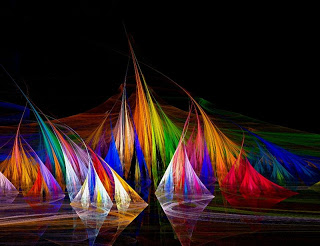
\includegraphics{img/Logo.jpg}\\ % Include a department/university logo - this will require the graphicx package

%----------------------------------------------------------------------------------------
%	DATE SECTION
%----------------------------------------------------------------------------------------

{\large \today}\\[1cm] % Date, change the \today to a set date if you want to be precise


%----------------------------------------------------------------------------------------

\vfill % Fill the rest of the page with whitespace

\end{titlepage}

\tableofcontents
\newpage

\section{Introducción}
Antes de comenzar a indagar en los fundamentos de la Teoría del Caos o en los fractales, debemos aclarar una serie de conceptos que aparecerán a lo largo de estos apuntes.

\begin{definition}[Sistema dinámico]\label{def:sistemaDinamico}
Un sistema dinámico es un sistema que consiste en un conjunto de estados, junto con una regla que determina el estado \emph{actual} en términos de los estados \emph{anteriores}.
\end{definition}

Los sistemas físicos en situación no estacionaria (es decir, los que varían con el tiempo) son ejemplos de sistemas dinámicos. También existen modelos económicos, matemáticos y de otros tipos que son sistemas abstractos y a la vez, son sistemas dinámicos.

Según las variables que intervienen en el sistema sean \textbf{discretas} (sólo tomen una serie de valores posibles) o \textbf{continuas} (pueden tomar cualquier valor dentro de un intervalo), así lo será el sistema.

Cuando definamos un sistema dinámico, exigiremos que la regla que lo rige sea determinista, es decir, una regla que nos permite conocer \emph{teóricamente} la evolución del sistema con total precisión. En particular, diremos que un sistema es \textbf{determinista} si es posible determinar su estado actual (p.e. la población de una cierta especie) \emph{solamente} a partir de los estados anteriores.

Es importante destacar el hecho de que los sistemas han de ser deterministas pues, de lo contrario, estaríamos hablando de procesos aleatorios, y por tanto, impredecibles. La \emph{idea clave} del concepto del Caos es que comprendemos el fenómeno y sabemos modelizarlo ``a la perfección'' pero el resultado futuro varía enormemente a partir de un pequeño cambio en los valores tomados del mundo real.


\begin{definition}[Teoría del Caos]
La teoría del Caos es la rama de las Matemáticas que estudia el comportamiento de sistemas dinámicos \emph{deterministas} muy sensibles a los datos iniciales.
\end{definition}

\begin{example}\label{example:Julia}
A modo de ejemplo podemos suponer un fenomeno que venga modelizado por la ecuación:
\[z_{n+1} = f(z_n) \text{ siendo } f(x) = x^2+1\]

Puesto que conocemos la ecuación que modela el fenómeno, queda claro que nos encontramos ante un sistema dinámico determinista, pues para todo valor de $n$ podemos calcular $z_{n+1}$.

Para un $n=11$, que no parece ser algo demasiado grande, siendo $z$ un número complejo, supongamos que cometemos un error muy pequeño, de la forma: $ε=10^{-5}+10^{-5}i$ al medir $z_0$.

En estas condiciones, la diferencia entre el valor obtenido y el original es
\[f^{11}(ε)=1.4 \cdot 10^{181} + 1.13\cdot 10^{174}\]

Este ejemplo será estudiado con más detalle al hablar de los conjuntos de Mandelbrot.
\end{example}

También es fundamental aclarar, aunque algunos lectores pueden tener ya una idea intuitiva, qué es un fractal.

\begin{definition}[Fractal]
Un fractal es un objeto geométrico cuya estructura básica, fragmentada o irregular, se repite a diferentes escalas.
\end{definition}

\section{Sistemas discretos}
\begin{definition}[Sistemas discretos]
Los sistemas dinámicos discretos son aquellos que sólo pueden tomar una serie de valores posibles.

Un reloj digital sería un sistema dinámico discreto mientras que un reloj analógico sería un sistema dinámico continuo.
\end{definition}

Para \emph{modelizar} los sistemas dinámicos discretos empleamos las ecuaciones en diferencias.

\subsection{Ecuaciones en diferencias.}

\begin{definition}[Ecuación en diferencias]
Una ecuación en diferencias es una expresión del tipo:
\[G(n,f(n),f(n+1),...,f(n+k))=0, \ \forall n \in \mathbb{Z}\]
donde $f$ es una función definida en $\mathbb{Z}$.
\end{definition}

\begin{example}
La ecuación en diferencias de primer orden:
\[X_{t+1} = F(X_t)\]
constituye un ejemplo de sistema dinámico determinista, siendo $F(x)$ una función conocida.
\end{example}

% Todo lo que viene a continuación viene de http://ltcconline.net/greenl/courses/204/firstOrder/differenceEquations.htm

A simple vista puede parecer que el ejemplo mencionado no es una ecuación en diferencias, puesto que no se aprecia ninguna derivada en la ecuación. No obstante, podemos escribir:
\[X'(t)=g(X(t)) \implies \lim_{h\to 0} \frac{X(t+h)-X(t)}{h}\]

Puesto que los valores posibles de $t$ y $h$ son enteros, lo más pequeño que puede ser $h$ sin llegar a ser $0$ es $h=1$ con lo que tenemos:
\[g(X(t))=X'(t)=X(t+h)-X(t)=ΔX(t) \implies X(t+h) = X(t) +ΔX(t) \implies \atop F(X(t)) = X(t) + ΔX(t)\]

Por tanto, encontrar la función $X(t)$ que resuelve el sistema planteado en el ejemplo es equivalente a resolver la ecuación:
\[X(t+1)=X(t)+ΔX(t)\]
que, claramente, es una ecuación en diferencias.


\subsection{Procesos de Verhulst. Period doubling, bifurcaciones.}
\subsection{Ecuación logística}
\subsection{$x=x^2+c$. Julia sets. Mandelbrot set.}

\subsubsection{Repaso de números complejos}
Antes de comenzar a hablar de los fractales de Julia y Mandelbrot se hace necesario dar una pequeña referencia sobre los números complejos. Básicamente podemos definir un número complejo como una expresión de la forma:
\[z=a +bi\]
Donde a y b son numeros reales, e i es la raiz cuadrada de -1.

Los números complejos se representan en un plano: \textbf{el plano complejo}, de manera que cada número complejo tiene asociado un punto del plano y viceversa. Es en esta identificación entre puntos del plano y números complejos en lo que se basa la representación de los fractales.

\subsubsection{Conjunto de Julia}
\begin{definition}[Conjunto de Julia]
Los \textbf{conjuntos de Julia}, así llamados por el matemático Gaston Julia, son una familia de conjuntos fractales que se obtienen al estudiar el comportamiento de los números complejos al ser iterados por una función.

Son conjuntos de Julia, por ejemplo, los formados por la familia cuadrática definida por la ecuación de recurrencia vista en el ejemplo \ref{example:Julia}:

\begin{equation}
z_{n+1} = z_n^2+c \text{ siendo } c \text{ un número complejo}
\end{equation}\label{eq:Julia}

\end{definition}

Para explicar los conjuntos de Julia nos basaremos en el ejemplo que acabamos de comentar, aunque puede realizarse una construcción equivalente con muchas otras funciones.

El conjunto de Julia que se obtiene a partir de esta función se denota \textbf{J$_c$}. Para construirlo, partiendo de un punto cualquiera $z_0$, aplicamos la ecuación \ref{eq:Julia} de manera iterativa obteniendo una serie de puntos del plano:
\[\begin{array}{l}
z_0=z_0\\
z_1=z_0^2+c \\
z_2 = z_1^2 + c \\
\vdots \\
z_{n+1} = z_n^2+c
\end{array}\]

Si esta sucesión queda acotada, entonces se dice que $z$ pertenece al conjunto de Julia de parámetro $c$, denotado por $J_c$; de lo contrario, si la sucesión tiende al infinito, $z$ queda excluido de éste.

Debido a la enorme cantidad de cálculos que se necesitaban para obtener la gráfica correspondiente, se tuvo que esperar hasta los años ochenta para poder representar estos conjuntos.

Algunos ejemplos de conjuntos de Julia aplicando diferentes valores de $c$ a la ecuación anterior están representados en la figura \ref{fig:Julia}

\begin{figure}[hbtp]
\centering
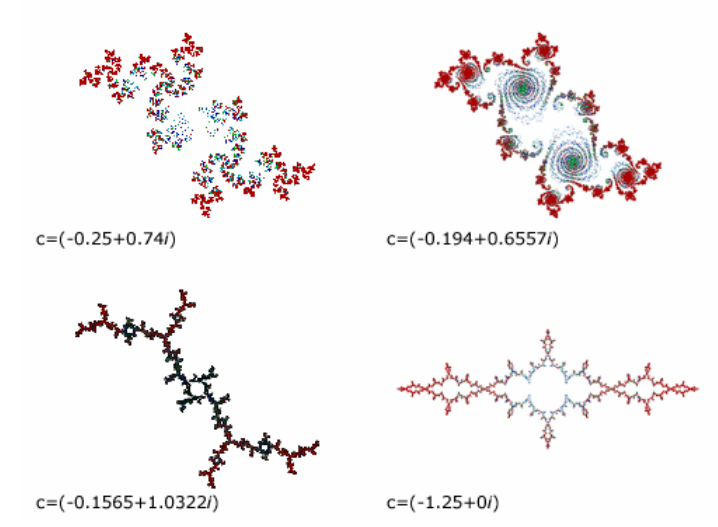
\includegraphics[width = 0.6\textwidth]{img/Julia_sets.png}
\caption{Ejemplos de conjuntos de Julia}
\label{fig:Julia}
\end{figure}

Puede demostrarse que si $|z_n| > 2$ entonces la sucesión diverge y el punto $z_0$ no pertenece al conjunto de Julia. Por lo tanto, basta encontrar un sólo término en la sucesión que verifique esta desigualdad para tener la certeza de que $z_0$ no está en el conjunto.

\subsubsection{Conjunto de Mandelbrot}
\begin{definition}
El conjunto de Mandelbrot es el más conocido de los conjuntos fractales y el más estudiado. Se conoce así en honor al matemático Benoît Mandelbrot (1924-2010), que investigó sobre él en los años setenta.

Mandelbrot modifica el proceso iterativo de Julia haciendo variable el punto $c$ y fijando el punto $z_0=0$. El conjunto de Mandelbrot es el conjunto de números complejos $c$ para los cuales la sucesión de puntos obtenida por el método iterativo:
\[\begin{array}{l}
z_0=z_0\\
z_1=z_0^2+c \\
z_2 = z_1^2 + c \\
\vdots \\
z_{n+1} = z_n^2+c
\end{array}\]
no tiende a infinito, es decir, está acotada.
\end{definition}

La figura \ref{fig:Mandelbrot} muestra la representación del conjunto de Mandelbrot obtenida si asignamos el color negro a los puntos $c$ que dan lugar a sucesiones acotadas y otros colores a los demás puntos, según lo rápido que tiendan al infinito.

\begin{figure}[hbtp]
\centering
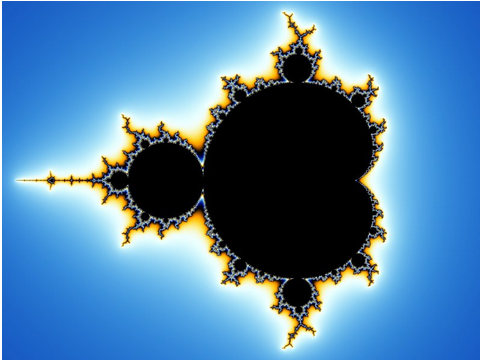
\includegraphics[width = 0.6\textwidth]{img/Mandelbrot_set.png}
\caption{Conjunto de Mandelbrot}
\label{fig:Mandelbrot}
\end{figure}

Si la constante $c$ fuera la misma para todos los puntos del dibujo y no dependiera de la posición, obtendríamos los llamados \emph{Conjuntos de Julia}. Hay uno diferente para cada punto del plano complejo. Estos conjuntos están completamente relacionados con el \emph{Conjunto de Mandelbrot}. Para cada punto de éste se puede decir que hay un conjunto de Julia. La figura \ref{fig:Mandelbrot-Julia} ilustra esta relación:

\begin{figure}[hbtp]
\centering
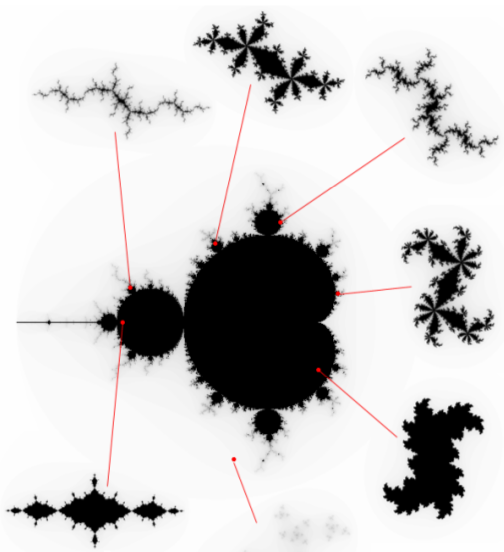
\includegraphics[width = 0.6\textwidth]{img/Mandelbrot-Julia.png}
\caption{Conjuntos de Julia asociados a cada punto del conjunto de Mandelbrot}
\label{fig:Mandelbrot-Julia}
\end{figure}

Queda claro pues que los conjuntos de Mandelbrot y Julia están estrechamente relacionados. El conjunto de Mandelbrot itera $z=z^2+c$ comenzando con $z = 0$ y variando el valor de $c$. El de Julia, por su parte, itera esa misma función, pero con valores fijos para $c$ y variando los de $z$. Cada punto $c$ en el conjunto de Mandelbrot especifica la estructura geométrica del conjunto de Julia correspondiente. Si $c$ está en el conjunto de Mandelbrot, entonces el de Julia será conectado (cerrado). De lo contrario, el conjunto de Julia será sólo una colección de puntos desconectados, trazados sobre una gráfica.

\subsection{Fractales/dimensión de Hausdorlf/dimensión fractal}
\subsection{Polvo de Cantor} No aparece en The Beauty of fractals (en algún otro libro de la bibliografía está).

%%%%%%%%%%%%%%%%%%%%%%%%%%%%%%%%%%%%%%%%%%%%%%%%%%%%%%%%%%
%%%%%%%%%%%%%%%%%%%%%%%%%%%%%%%%%%%%%%%%%%%%%%%%%%%%%%%%%%
%%%%%%%%%%%%%%%%%%%%%%%%%%%%%%%%%%%%%%%%%%%%%%%%%%%%%%%%%%
%%%%%%%%%%%%%%%%%%%%%%%%%%%%%%%%%%%%%%%%%%%%%%%%%%%%%%%%%%
%%%%%%%%%%%%%%%%%%%%%%%%%%%%%%%%%%%%%%%%%%%%%%%%%%%%%%%%%%
%%%%%%%%%%%%%%%%%%%%%%%%%%%%%%%%%%%%%%%%%%%%%%%%%%%%%%%%%%
%%%%%%%%%%%%%%%%%%%%%%%%%%%%%%%%%%%%%%%%%%%%%%%%%%%%%%%%%%
%%%%%%%%%%%%%%%%%%%%%%%%%%%%%%%%%%%%%%%%%%%%%%%%%%%%%%%%%%
%%%%%%%%%%%%%%%%%%%%%%%%%%%%%%%%%%%%%%%%%%%%%%%%%%%%%%%%%%

\section{Sistemas continuos}
% Tiempo estimado de esta parte: 70 min.\\
% Referencia
% \begin{itemize}
% \item CHAOS: An introduction to dynamical systems temas 7,8,9 y 11.
% \item Elegant Chaos
% \end{itemize}

\subsection{Sistemas dinámicos deterministas, ecuaciones diferenciales}

Los sistemas dinámicos continuos deterministas, definidos en \ref{def:sistemaDinamico}, vienen modelizados por ecuaciones diferenciales.

En lugar de expresar el estado actual en función de un estado anterior, las ecuaciones diferenciales tratan de expresar la \emph{tasa de cambio} del estado actual en función del estado actual. La tasa de cambio de una cierta función es su \emph{derivada}. Tenemos la siguiente definicón general de ecuación diferencial.

\begin{definition}[Ecuación diferencial]
Una ecuación diferencial es una fórmula matemática que relaciona una función con sus derivadas.
\end{definition}

\begin{example}[Ecuación del calor]\label{ex:calor}
Un ejemplo de este tipo de dependencia es la \emph{Ley del calor de Newton}. Si consideramos $x$ como la diferencia de temperatura entre el objecto caliente y la temperatura ambiente del aire que lo rodea, la tasa de cambio de esta diferencia de temperatura es inversamente proporcional a la diferencia de temperatura. En términos de ecuaciones diferenciales, diremos:
\begin{equation}
x'(t) = ax(t)~~~con~~ a<0
\end{equation}

La solución de esta ecuación viene dada por:
\begin{equation}
x(t) = c\cdot e^{at}
\end{equation}

Esto quiere decir que la diferencia de temperatura $x(t)$ decrece exponencialmente con el tiempo $t$. Se trata de una ecuación  de \emph{primer orden}, puesto que el \emph{orden} de la derivada más alto que aparece es el de la \emph{primera} derivada, y \emph{lineal} porque la relación entre las funciones $x'(t)$ y $x(t)$ en la ecuación es \emph{lineal}.
\end{example}

En el siguiente ejemplo, veremos un caso de ecuación diferencial \emph{de segundo orden} \emph{no lineal}.

\begin{example}[Péndulo]
En este caso estudiaremos el movimiento de un péndulo \emph{bob}, el movimiento de un péndulo que tiene en su extrem un peso y que cuelga de un soporte que limita su movimiento a lo largo de un círculo. La aceleración que experimenta este péndulo es tangente a la dirección del movimiento y proporcional a la componente de la fuerza gravitatoria sobre la dirección tangencial. Si representamos con $x(t)$ la posición angular (es decir, la razón entre la longitud del arco que forma el péndulo con la vertical y la longitud del péndulo), entonces la relación entre su derivada segunda y ésta viene dada por:
\begin{equation}
x''(t) = -\sin x(t)
\end{equation}

Esta ecuación es una de las más importantes en ciencia y se trata de una ecuación de \emph{segundo orden}, puesto que el \emph{orden} de la derivada más alto que aparece es el de la \emph{segunda} derivada, y \emph \emph{no lineal}, porque la relación entre las funciones $x''(t)$ y $x(t)$ en la ecuación es \emph{no lineal}.
\end{example}


En ambos ejemplos, buscamos soluciones de la forma $x(t)$ donde $t$ denota el tiempo y $x(t)$, por tanto, una cierta magnitud física que varía en función del tiempo: en el primer ejemplo, la diferencia de temperatura; en el segundo ejemplo, la posición angular. Es por eso que consideramos que $x(t)$ es una variable \emph{dependiente}.


\begin{definition}[Ecuación diferencial autónomas]
Si la variable \emph{independiente} $t$ no aparece explicítamente en la ecuación, como es el caso en los dos ejemplos anteriores, hablaremos de ecuaciones diferenciales \textbf{autónomas}. Si $t$ aparece explícitamente en la ecuación como es el caso de la ecuación del \emph{péndulo amortiguado} (el columpio):
\begin{equation}
x''(t) = -cx'(t)-\sin x(t)+\rho~\sin t
\end{equation}
entonces hablaremos de ecuaciones diferenciales \textbf{no autónomas}.
\end{definition}

Recapitulando las nociones vistas hasta ahora tendríamos la siguiente clasificación de las ecuaciones diferenciales:

\begin{itemize}
\item Según el orden de las derivadas que aparezcan en la expresión:
	\begin{itemize}
	\item Primer orden
	\item Segundo orden
	\item ...
	\end{itemize}
\item Según la relación entre la función $x$ y sus derivadas
	\begin{itemize}
	\item Lineales
	\item No lineales
	\end{itemize}
\item Según si aparece explicítamente la variable $t$ en la ecuación
	\begin{itemize}
	\item Autónomas
	\item No autónomas
	\end{itemize}
\end{itemize}

Si recuperamos el ejemplo \ref{ex:calor}, teníamos que las soluciones eran de la forma:
\begin{equation}
x(t) = c \cdot e^{at}
\end{equation}

La $c$ es una constante en $\mathbb{R}$, cuyo valor dependerá del punto inicial que tomemos, es decir, la ecuación diferencial planteada en \ref{ex:calor} tiene \emph{infinitas} soluciones, a menos que especifiquemos un \emph{valor inicial} $x(0)$.

En el momento en que definimos un valor inicial $x(0)=x_0$ tenemos:
\[x(0)=c\cdot e^0=c \implies c=x_0 \implies x(t) = x(0)\cdot e^{at}\]

Así, estamos \emph{seleccionando} una de las soluciones dentro de la familia de soluciones.


% No se que aparece en la pagina que decías, pero yo me dibujo aquí la familia de funciones que creo que hay que poner xd
\begin{center}
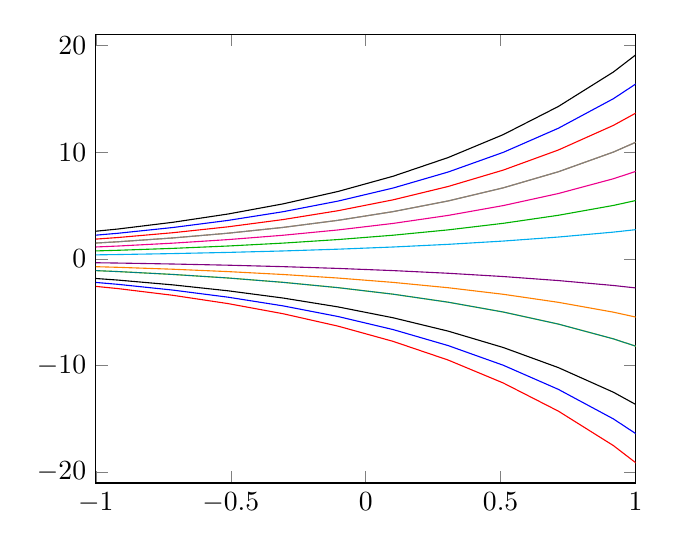
\begin{tikzpicture}
\begin{axis}[xmin=-1, xmax=1, samples=50, cycle list name=color list]
  \addplot (x,-7*e^x);
  \addplot (x,-6*e^x);
  \addplot (x,-5*e^x);
  \addplot (x,-3*e^x);
  \addplot (x,4*e^x);
  \addplot (x,-3*e^x);
  \addplot (x,-2*e^x);
  \addplot (x,-1*e^x);
  \addplot (x,e^x);
  \addplot (x,2*e^x);
  \addplot (x,3*e^x);
  \addplot (x,4*e^x);
  \addplot (x,5*e^x);
  \addplot (x,6*e^x);
  \addplot (x,7*e^x);
\end{axis}
\end{tikzpicture}
\captionof{figure}{Familia de funciones de la forma $x(t)=x(0)e^t$}
\end{center}

En nuestro caso, podemos establecer:

\begin{equation}
x(0) = x_0
\end{equation}

y por tanto, la solución particular de nuestro problema sería:

\begin{equation}
x(t) = x_0e^{at}.
\end{equation}

En general, a los problemas experesados en forma de ecuación diferencial más dato inicial, los denominaremos \textbf{problemas de valor inicial}.\newline
Es el momento de introducir el concepto de \emph{espacio de fases}, que nos permitirá estudiar el comportamiento cualitativo de nuestras soluciones, e incluso, será la idea a la que nos aferremos para obtener las soluciones en casos más complicados.

\subsection{Espacio de estados/fases}

Un concepto muy útil a la hora de trabajar con ecuaciones diferenciales son los \textbf{diagramas de fases}, pues nos permite conocer de manera inequívoca el estado de nuestra sistema en cualquier tiempo futuro.

Tomemos la ecuación diferencial
\[y(x)'=f(y(x))\]
donde la función $f$ viene dada por la siguiente gráfica

\begin{figure}[hbtp]
\centering
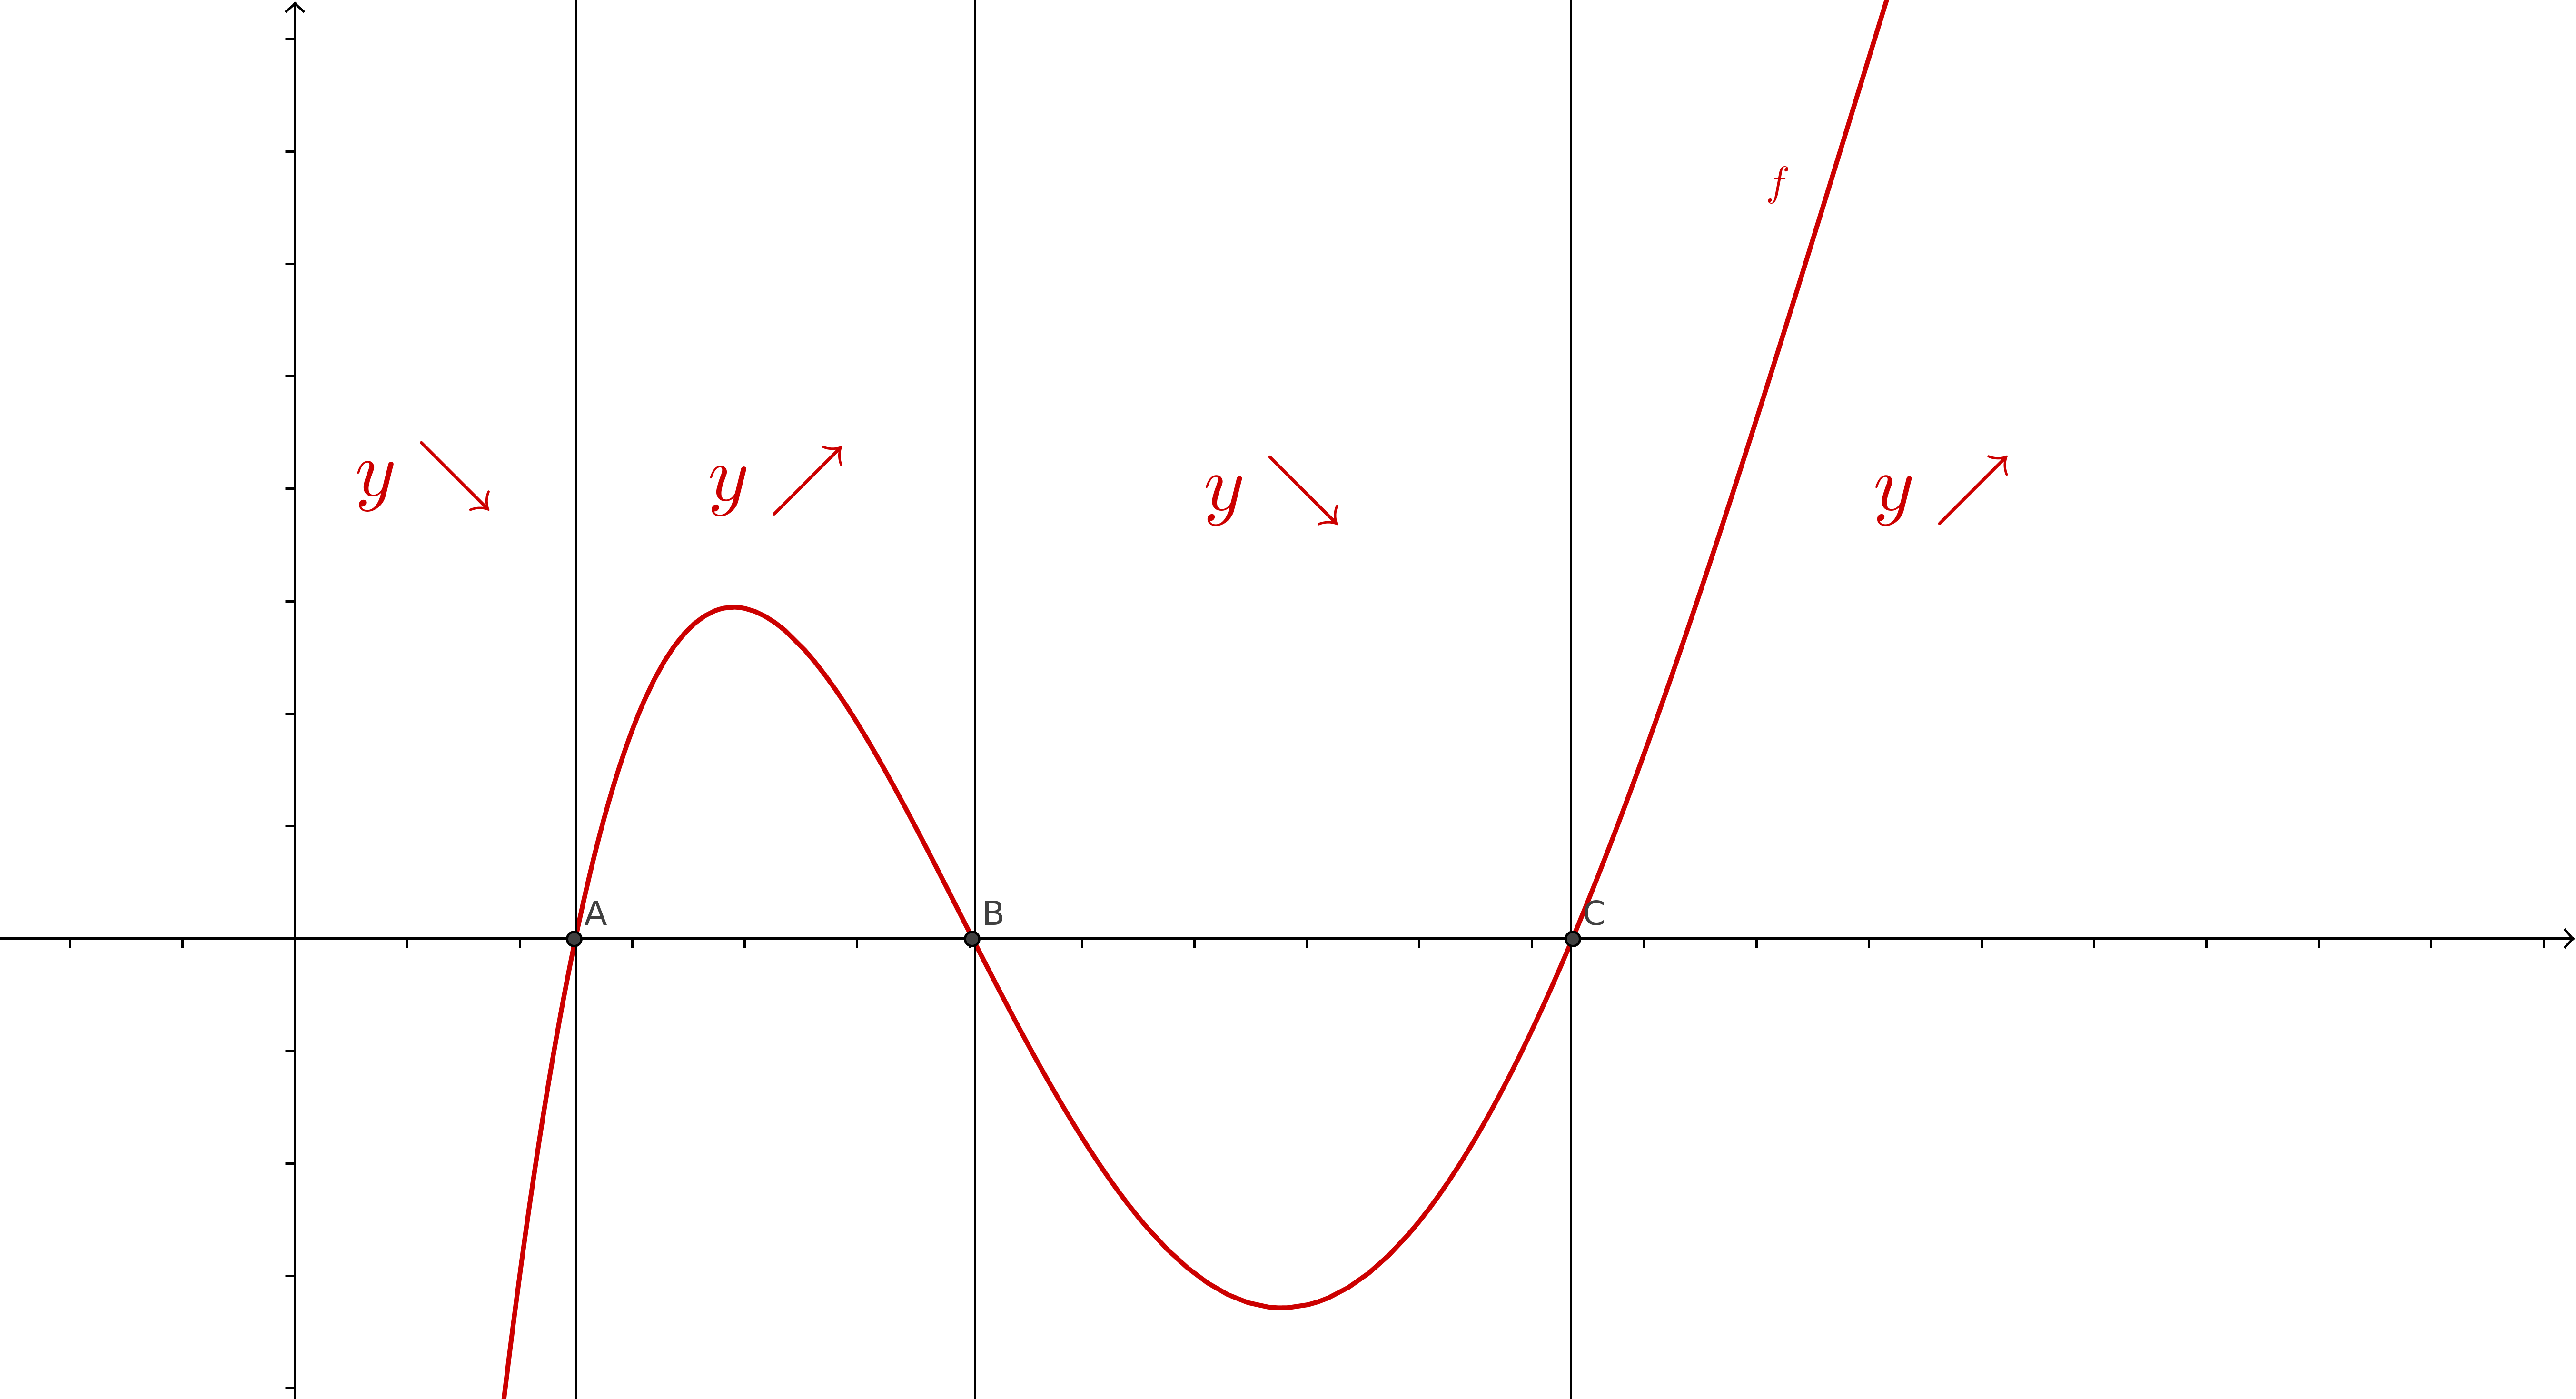
\includegraphics[width = 0.6\textwidth]{img/propiedades-autonomas.png}
\end{figure}

Podemos observar que si nos situamos ``a la izquierda de $a$'' o ``entre $b$ y $c$'' la función $y$ es decreciente. Del mismo modo, si nos situamos ``entre $a$ y $b$'' o ``a la derecha de $c$'' la función será creciente mientras que en los puntos $a, b$ y $c$ la función ni crece ni decrece. Esta información queda recogida en el siguiente diagrama de fases:

\begin{figure}[hbtp]
\centering
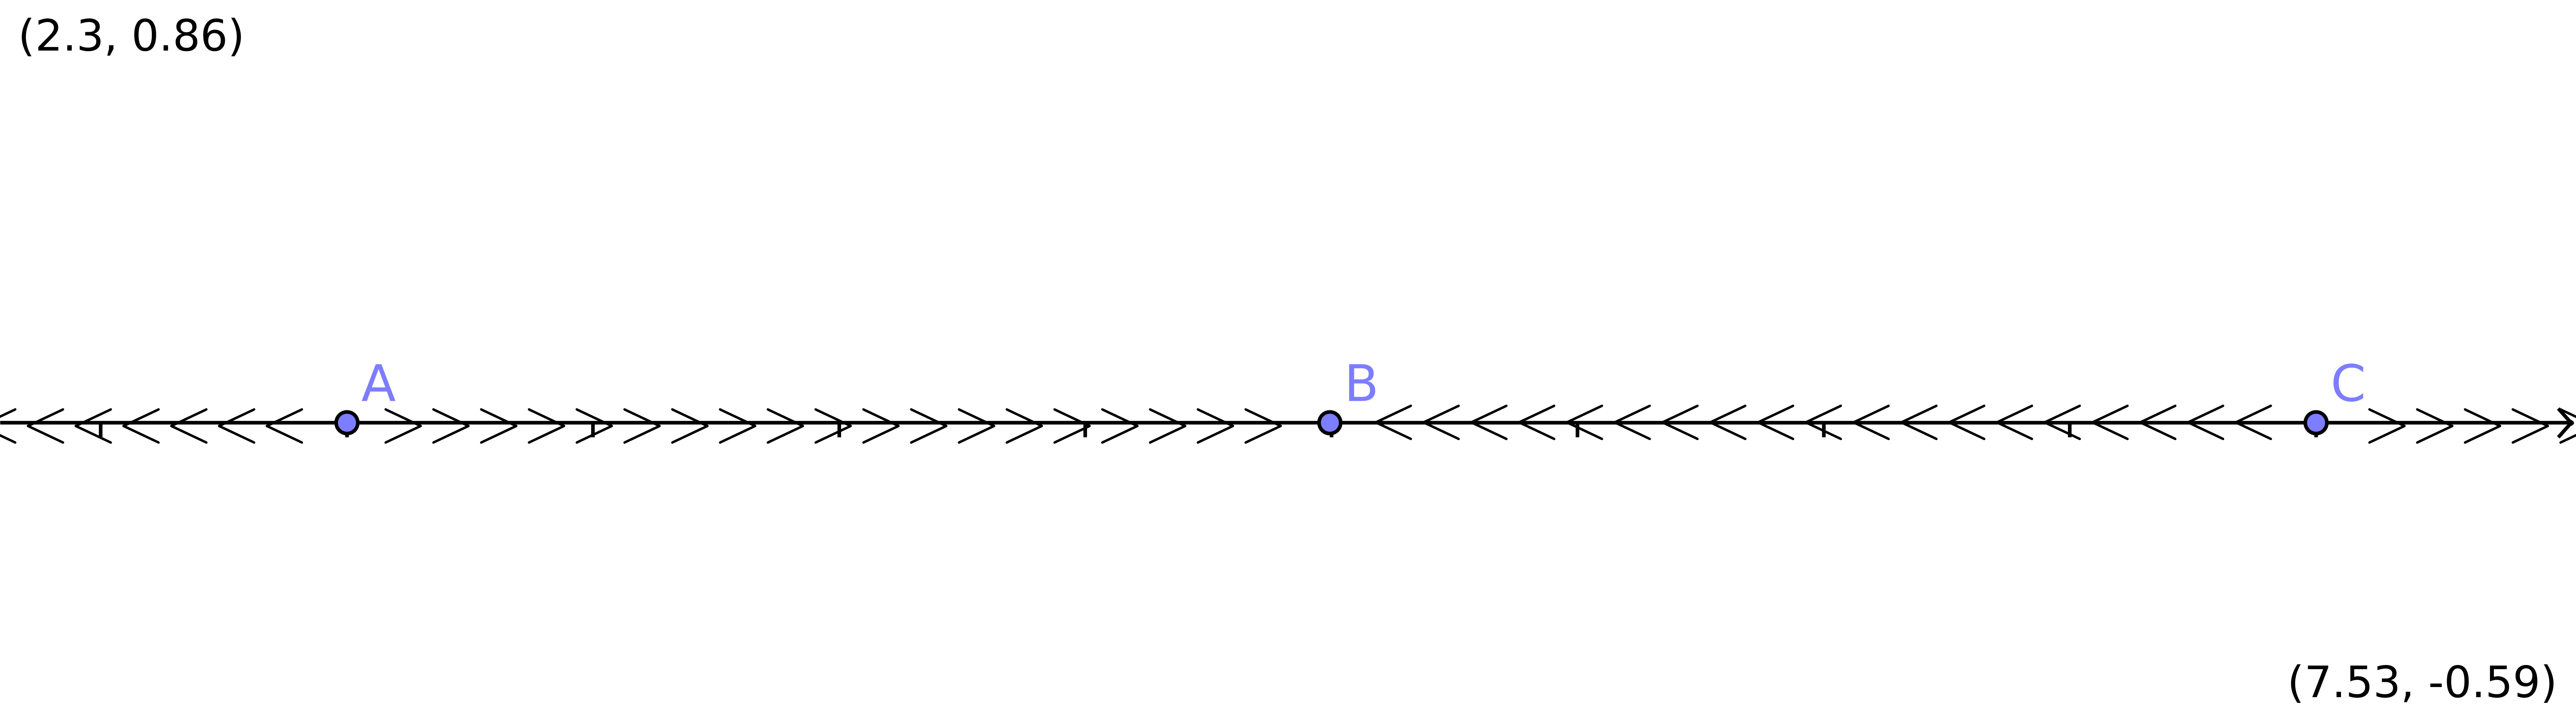
\includegraphics[width = 0.6\textwidth]{img/diagrama-fases.png}
\end{figure}

En este caso diremos que $a$ y $c$ son puntos \textbf{inestables} pues una pequeña perturbación hará que nos alejemos de ellos. Igualmente, diremos que $b$ es un punto \textbf{estable} porque una pequeña perturbación hará que volvamos de nuevo a desplazarnos hacia $b$.

\begin{example}
Retomamos el ejemplo \ref{ex:calor} considerando un valor $a=-1$. Ya vimos que la solución a la EDO era:
\[x(t) = x(0)\cdot e^{-t}\]

En esta ocasión, estudiando el signo de la derivada $x'(t)=ax(t)$ vemos que la la pendiente sólo se anula en $x(t)=0$ y que una vez que la función $x(t)$ toma un valor positivo empieza a decrecer del mismo modo que crece al encontrar un valor negativo. Por tanto tenemos un punto estable en $x(t)=0$. Esto provoca que un pequeño error en la aproximación del dato inicial, cuanto tomamos $t$ grande, no nos aleje mucho del valor real.

Es decir, si tomamos por error $\tilde{x}_0 = x_0 + ε$, estamos cometiendo un error ε en la medida del dato inicial, lo que nos lleva a un error:
\[x(t)-\tilde{x}(t) = x_0\cdot e^{-t} - \tilde{x}_0\cdot e^{-t} = e^{-t}\cdot ε\]
al evaluar la función. Puesto que tenemos una exponencial en el denominador, por mucho error ε que hayamos cometido, al final, este será ``despreciable''.
\end{example}

\begin{example}
Repitamos el mismo ejemplo con $a=1$. En este caso tendremos:
\[x(t) = x(0)\cdot e^{t}\]

Imitando el ejemplo anterior es trivial comprobar que no hay ningún punto estable.

Por tanto, si tomamos por error $\tilde{x}_0 = x_0 + ε$, estamos cometiendo un error ε en la medida del dato inicial, lo que nos lleva a un error:
\[x(t)-\tilde{x}(t) = x_0\cdot e^{t} - \tilde{x}_0\cdot e^{t} = e^{t}\cdot ε\]
al evaluar la función. Puesto que tenemos una exponencial el error cometido se dispara.
\end{example}

\subsection{Sistemas de ecuaciones no lineales}
Hasta ahora la tarea ha sido relativamente sencilla, sin embargo, no podemos decir lo mismo cuando estudiamos sistemas dinámicos \emph{no lineales}. La mayoría de los sistemas no lineales de ecuaciones diferenciales no pueden ser resueltos de manera explícita, es decir, las soluciones a dicho sistema no se pueden obtener mediante cálculo. Usaremos métodos geométricos que nos revelarán propiedades cualtitativas de las soluciones: Para qué valores del dato inicial las soluciones son crecientes? Para qué valores son decrecientes?,...

Utilícemos un ejemplo para ilustrar los conceptos siguientes: Supongamos que trabajamos con un modelo para estudiar la evolución de una cierta población. Es común, en este caso, utilizar la función \emph{logística} de la población:

\begin{equation}
x'(t) = a\cdot x(t)(1-\frac{x(t)}{K})~~~~con~~a>0~~yK>0
\end{equation}
A esta ecuación la llamamos \emph{ecuación diferencial logística}. En ese caso, $x(t)$ mide la población de una cierta especie. Llamamos $K$ al valor de la población \emph{limitante}, aquel a partir del cual la población deja de crecer y, de hecho decrece, por sobrepoblación.

Este tipo de comportamiento solo puede ser modelado mediante una ecuación no lineal. Ahora nos preguntamos: Es posible predecir para qué valores iniciales la población crecerá? Y para que valores sólo decrecerá?

En la siguiente gráfica observamos las soluciones de la ecuación diferencial logística:\newline

GRÁFICA SOLUCIONES.\newline

Con lo que hemos visto sobre puntos estables e inestables, le resultará sencillo al lector detectar que en $x=1$ tenemos un punto estable, mientras que en $x=0$, tenemos un punto inestable. Decimos que ambas soluciones $x(t) = 0$ y $x(t) = 1$ son \textbf{soluciones de equilibrio}.

Ahora podemos resolver las preguntas planteadas anteriormente. La población crecerá siempre la población sea positiva y estrictamente menor que $K$. Mientras que decrecerá siempre que sea superior a $K$. Por otro lado, las soluciones que corresponden con valores negativos de la población y que \emph{explotan} (se van a infinito) en tiempo finito, afortunadamente, pueden descartarse pues no tienen sentido físico.\newline

OPCIONALMENTE, PODEMOS MOSTRAR EL DIAGRAMA DE FASES DE ESTA ECUACIÓN.\newline

Para poder resolver sistemas de ecuaciones a partir de sus gráficas, nos basamos en los siguientes 3 conceptos importantes:

\begin{itemize}
\item \textbf{Existencia de solución} Para cada punto $(t,x)$ de la gráfica existe una  solución $x(t)$ que pasa por ese punto. La pendiente de dicha solución viene dada por la ecuación diferencial en ese punto.
\item \textbf{Unicidad de la solución} Para cada punto $(t,x)$ de la gráfica únicamente pasa una solución.
\item \textbf{Dependencia continua} Dada una cierta solucion $x(t)$ para un cierta condición inicial, las soluciones próximas en un cierto entorno del dato inicial permanecen próximas a lo largo de intervalos cortos de tiempo.
\end{itemize}

El concepto de dependencia continua no debe ser confundido con el de dependencia \emph{sensible} de las condiciones iniciales, también conocido como \textbf{efecto mariposa}. Éste hace refencia a la propiedad de ciertos sistemas dinámicos no lineales en los que una pequeña variación en los datos iniciales resulta en grandes variaciones en estados futuros tras un largo período de tiempo. Esta es la característica más importante de los \textbf{sistemas caóticos}.

\subsection{Oscilaciones}

\begin{definition}[Ecuación diferencial oscilante]
Decimos que una ecuación diferencial es oscilante cuando tiene infinitos puntos críticos. Un ejemplo de ecuación de este tipo es
\[x''(t)+x(t)=0\]
de la que $x(t)=\sin(t)$ es una solución.
\end{definition}

Con este tipo de ecuaciones nos encontramos con que hay numerosos puntos de estabilidad.

Sabemos que un pequeño error respecto al dato inicial, si este era el único punto estable, no era un problema puesto que la solución se acababa aproximando bastante a la estabilidad.

No obstante, si tenemos varios puntos de estabilidad la duda que nos surge es, ¿De qué solución real no se distancia mucho el valor que calculemos?

\subsection{Sistemas disipativos: atractores}
\subsection{Flujos, compresibles o no}

\subsection{Atractores extraños: caos}
El término ``atractor'' resulta en si mismo difícil de definir de manera formal y rigurosa. De manera informal un \textbf{atractor} es un conjunto hacia el que todas las trayectorias cercanas convergen. Los puntos fijos y los ciclos estables son ejemplos de atractores.

\begin{definition}[Atractor]
Un atractor es un conjunto cerrado, $A$, con las siguientes propiedades:
\begin{itemize}
\item Es un conjunto invariante, es decir, toda trayectora $\vec{x}(t)$ que empiece en el conjunto nunca sale de él.
\[\vec{x}(0) \in A \implies \vec{x}(t) \in A \ \forall t\]
\item Hay un conjunto abierto, $U$, que contiene a $A$ para el que toda trayectoria que comience en $U$ tiende al conjunto $A$.
\[\exists U \text{ abierto t.q. } \forall \vec{x}, \vec{x}(0) \in U \implies \lim_{t\to \infty}\text{distancia}(\vec{x}(t),A) = 0\]
\item $A$ es el conjunto más pequeño para el que se cumplen las propiedades anteriores.
\end{itemize}
\end{definition}

\begin{example}
Si consideramos el sistema bidimensional
\[\begin{array}{l}
x'(t) = x(t)-x^3(t) \\
y'(t) = -y(t)
\end{array}\]
podemos ver fácilmente que su plano de fases será el mostrado en la figura \ref{fig:planoFasesAtractorEjemplo}
\begin{figure}[H]
\centering
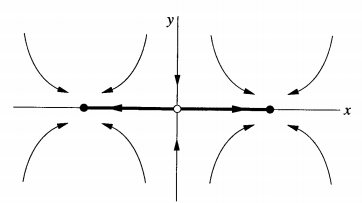
\includegraphics[width = 0.6\textwidth]{img/atractorExample.png}
\caption{Plano de fases asociado al sistema descrito en el ejemplo}
\label{fig:planoFasesAtractorEjemplo}
\end{figure}

Considerando el punto $(1,0)$ podemos observar que cumple las dos primeras propiedades de la definición de atractor. Sin embargo, no cumple la última propiedad, puesto que hay otro punto más que también satisface las propiedades necesarias.

Así, en este caso concreto, el atractor sería el conjunto
\[A=\{(\pm 1, 0)\}\]
\end{example}

\begin{definition}[Atractor extraño]
Un atractor extraño es un atractor que muestra una clara y sensible dependencia de las condiciones iniciales. Estos atractores fueron llamados \emph{extraños} en un primer momento debido a que, a menudo, son conjuntos fractales.

Actualmente, sus propiedades geométricas se consideran menos importantes que las propiedades dinámicas relacionadas con la dependencia con los datos iniciales.
\end{definition}

Es la sensibilidad del atractor respecto a los datos iniciales lo que nos lleva de nuevo al concepto de \emph{caos}, pues dificulta la predicción de valores futuros a partir de los datos actuales.

\subsection{Ecuaciones de Lorenz}
\begin{definition}[Ecuaciones de Lorenz]
En 1963 Lorenz desarrolló un sistema de ecuaciones tridimensional que modelizaba, de manera extraordinariamente simple, la convección en forma de anillos que parece ocurrir a veces en la atmósfera terrestre.

El sistema descrito por Lorenz fue:
\[\begin{array}{l}
x'(t) = σ(y(t)-x(t)) \\
y'(t) = rx(t)-y(t)-x(t)y(t)\\
z'(t) = x(t)y(t)-bz(t)
\end{array}\]
donde σ es el \textbf{número de Prandtl}, que representa la viscosidad/conductividad térmica, $r$ es el \textbf{número de Rayleigh}, que representa la diferencia de temperatura entre base y tope y $b$ es la razón entre la longitud y altura del sistema.
\end{definition}

Lorenz descubrió que este sistema de apariencia tan sencilla escondíga un comportamiento realmente caótico. Las soluciones oscilaban de manera irregular, sin repetirse nunca el mismo patrón pero manteniéndose siempre dentro de una región limitada del plano de fases. Como puede verse en la figura \ref{fig:Lorenz} la solución de las ecuaciones da lugar a un complicado conjunto \emph{con forma de mariposa} conocido hoy en día como \textbf{atractor extraño}. A diferencia de los puntos fijos estables, el \textbf{atractor extraño} no es un punto ni una curva ni si quiera una superficie, es un \emph{fractal} con dimensión fractal entre 2 y 3.

\begin{figure}[hbtp]
\centering
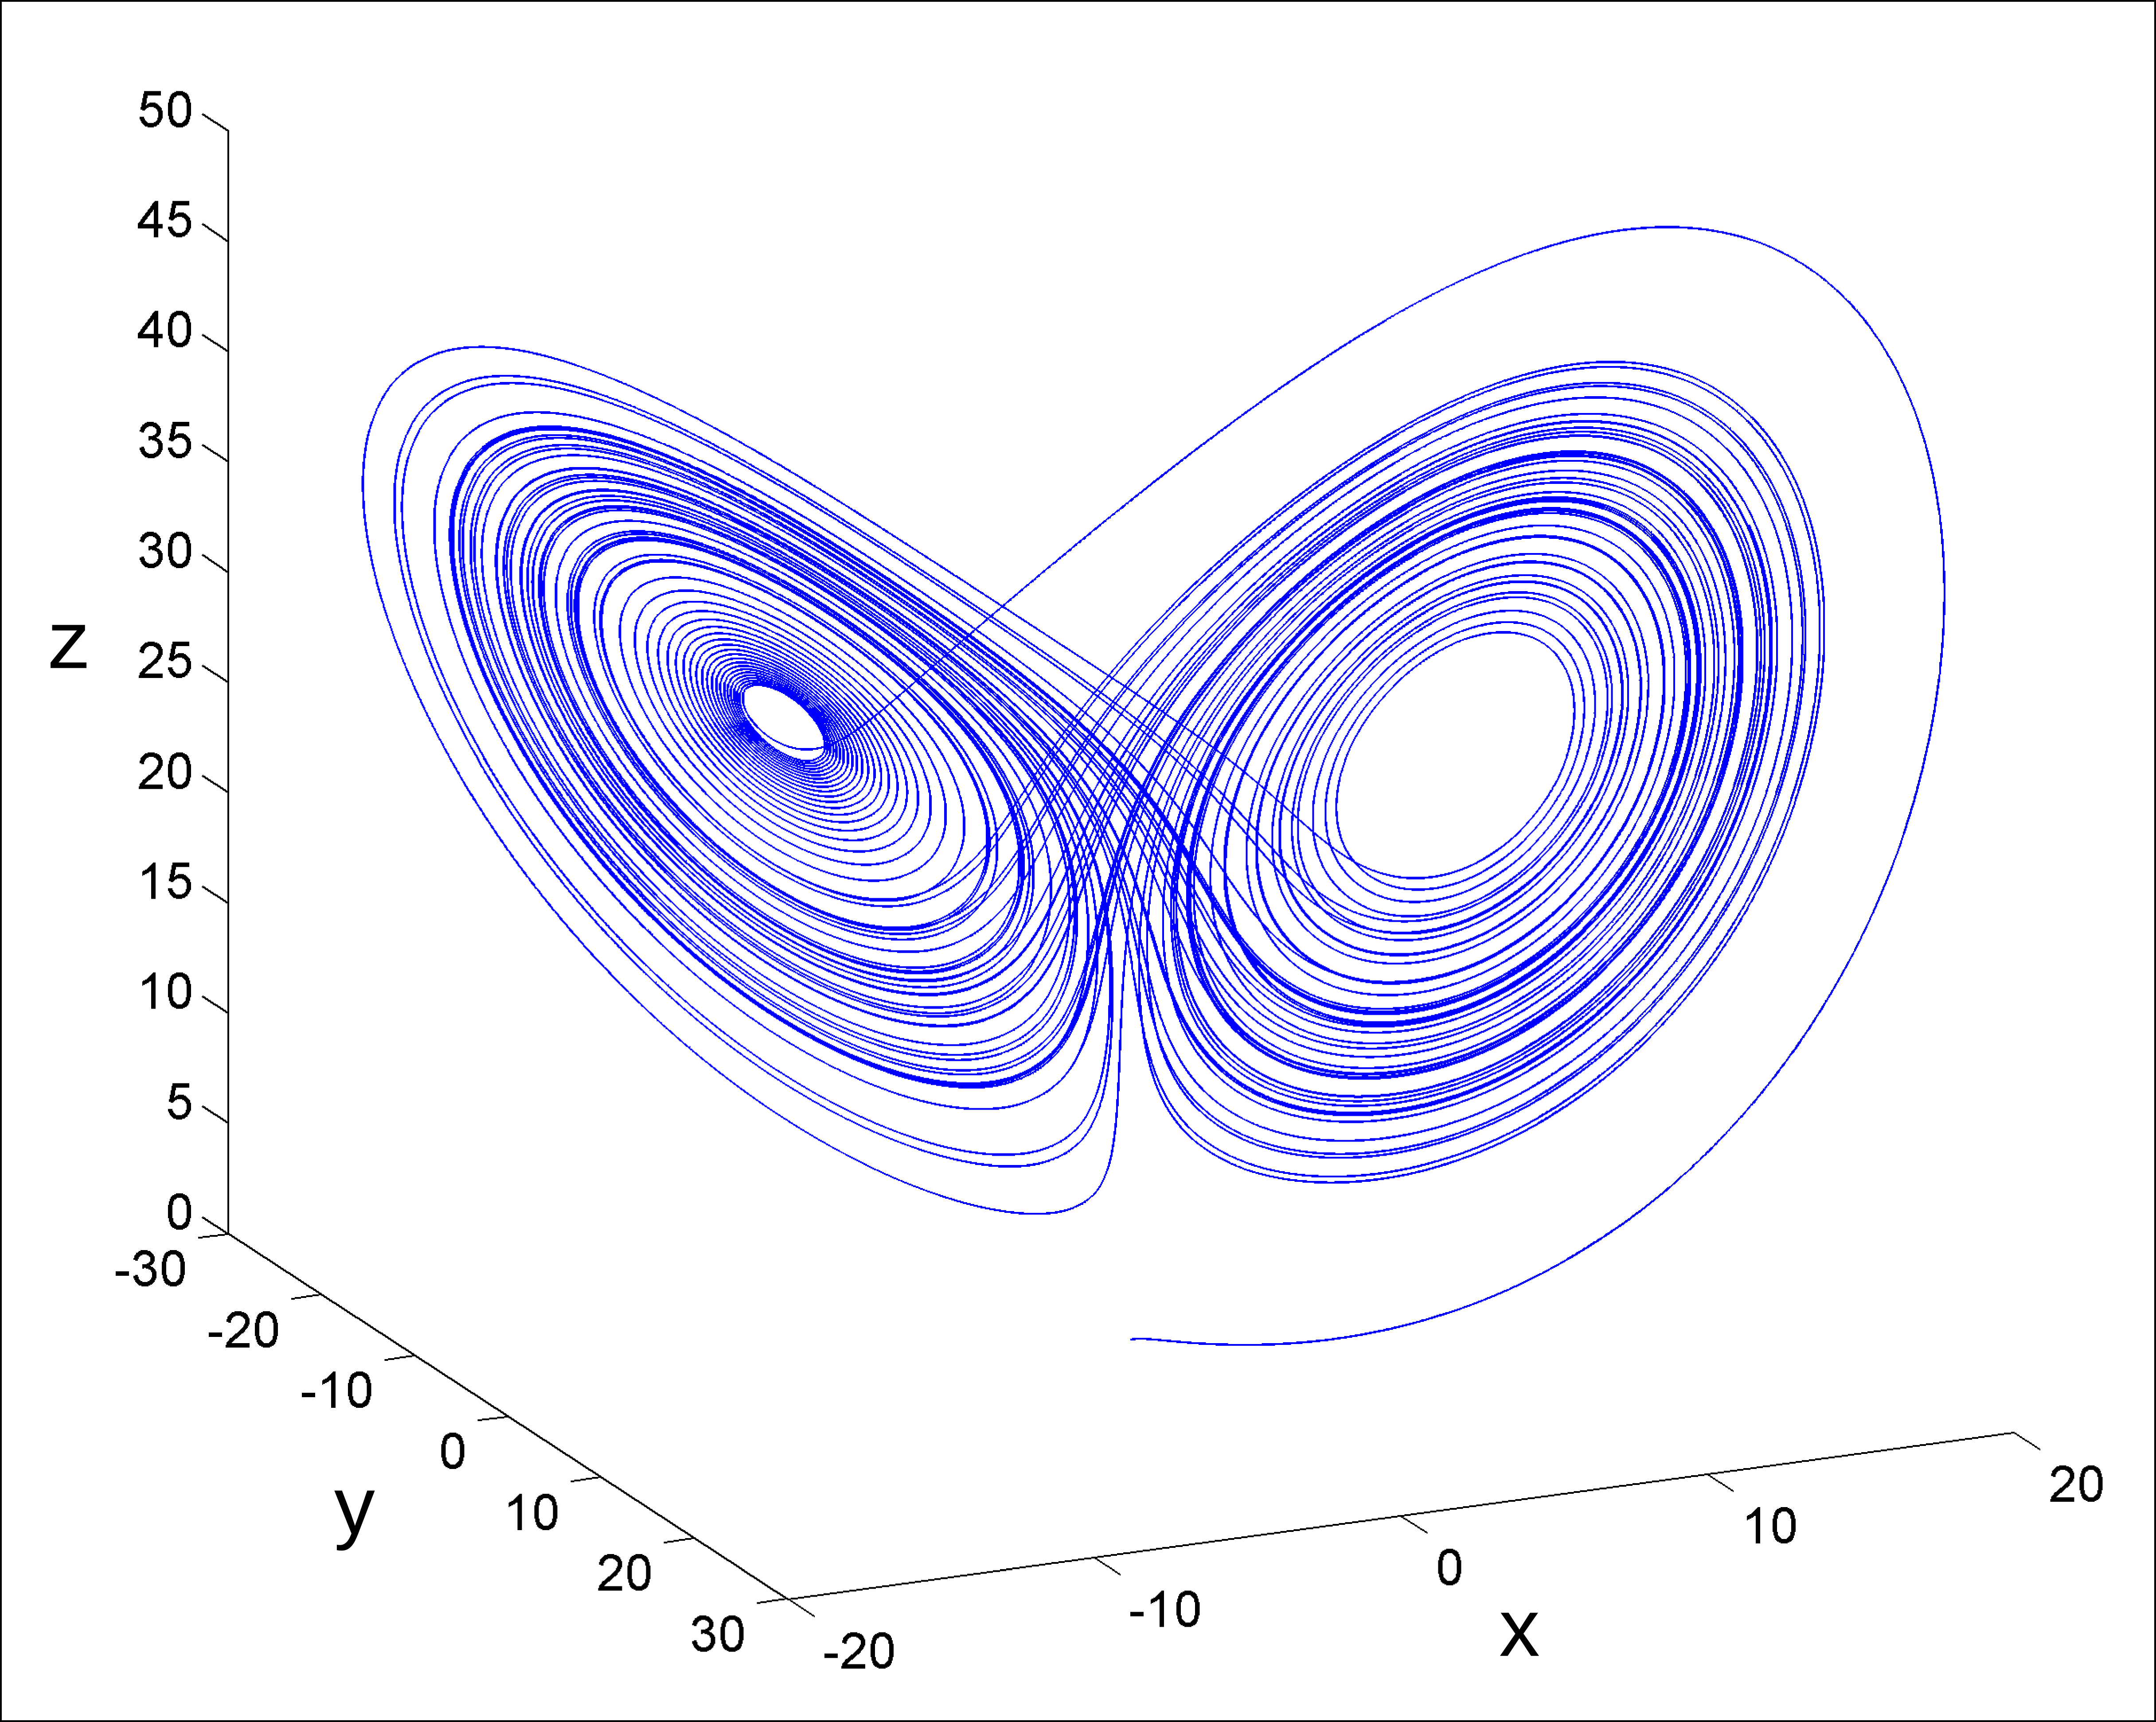
\includegraphics[width = 0.6\textwidth]{img/Lorenz.png}
\caption{Representación tridimensional de la solución de las ecuaciones de Lorenz}
\label{fig:Lorenz}
\end{figure}

\subsubsection{Algunas propiedades de las ecuaciones de Lorenz}
Lorenz publicó un artículo donde llevaba a cabo un análisis muy detallado de sus ecuaciones. Llevó el análisis tan lejos como pudo empleando ténicas estandarizadas pero, una vez llegado a cierto punto, se topó con lo que parecía un \emph{paradoja}. Una a una fue eliminando todas las posibilidades acerca del comportamiento del sistema a largo plazo.

Probó que, dentro de un cierto rango de parámetros, el sistema no tendría puntos fijos estable ni cilcos finitos estables. No obstante, también demostró que la ssoluciones no salían de una cierta región \emph{delimitada} y que, llegado a cierto punto, se veían atraídas hacia un conjunto de volumen cero. Este conjunto es lo que se conoce como \textbf{atractor extraño}.

Veamos por encima las propiedades del sistema que Lorenz estudió en su famoso artículo.

\begin{itemize}
\item \textbf{No linearidad}
El sistema de Lorenz presenta dos términos no lineales: $x(t)y(t)$ y $x(t)z(t)$.

\item \textbf{Simetría}
Si reemplazamos los términos $x(t)$ e $y(t)$ por $-x(t)$ y $-y(t)$ respectivamente obtenemos un sistema equivalente:
\[\begin{array}{l}
-x'(t) = -σ(y(t)-x(t)) \\
-y'(t) = -rx(t)+y(t)-x(t)y(t)\\
z'(t) = x(t)y(t)-bz(t)
\end{array}\]

Es decir, si $(x(t),y(t),z(t))$ es una solución también lo será $(-x(t),-y(t),z(t))$.

\item \textbf{Contracción de volumen}
El sistema de Lorenz es \emph{disipativo}: el volumen en el plano de fases se contrae. Para comprender esto lo primero que debemos hacer es ver cómo evoluciona este volumen.

Para cualquier sistema tridimensional $\vec{x}'(t) =f(\vec{x}(t))$, consideramos una superficie cerrada $S(t)$ de volumen $V(t)$ en el plano de fases. Consideremos ahora los puntos de $S(t)$ como puntos iniciales para diferentes trayectorias y veamos su evolución durante un instante de tiempo infinitesimal $dt$. Tras este tiempo $S(t)$ se convierte en una nueva superficie $S(t+dt)$.

La figura \ref{fig:volumen2D} representa en dos dimensiones la situación recien descrita.
\begin{figure}[hbtp]
\centering
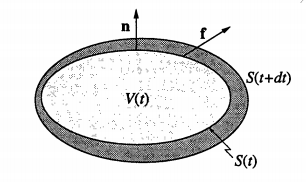
\includegraphics[width = 0.6\textwidth]{img/volumen2D.png}
\caption{Evolución con el tiempo de la superficie y del volumen contenido en su interior, siendo \textbf{n} el vector normal a la superfice $S(t)$}
\label{fig:volumen2D}
\end{figure}

El volumen encerrado por la nueva superficie derrada puede escribirse como
\[V(t+dt)=V(t) + \int_S (f\cdot \text{\textbf{n}}\ dt)\ dA\]

Puesto que
\[V'(t)=\frac{V(t+dt)-V(t)}{dt} = \int_S f\cdot \text{\textbf{n}}\ dA\]

Aplicando el teorema de divergencia podemos reescribir la integral como:
\[V'(t) = \int_V \nabla \cdot f \ dV \]
siendo, para el sistema de Lorenz
\[\nabla \cdot f = \frac{\partial}{\partial x}[σ(x-y)] + \frac{\partial}{\partial y}[rx-y-xy] + \frac{\partial}{\partial z}[xy-bz] = -σ-1-b < 0\]

Puesto que la divergencia es constante, la ecuación de la derivada del volumen queda
\[V'(t) = -(σ+1+b)V(t) \implies V(t) = V(0)e^{-(σ+1+b)t}\]
con lo que queda claro que el volumen de crece de manera exponencial.

\item \textbf{Puntos fijos}
El sistema de Lorenz tiene ``dos tipos de puntos fijos''.

Por un lado tenemos el punto fijo $(0,0,0)$ que lo es para cualquier combinación de parámetros que decidamos tomar. Por otro, tenemos puntos fijos que dependen de los parámetros seleccionados. Así
\[(\pm \sqrt{b(r-1)},\pm \sqrt{b(r-1)},r-1) \text{ para } r>1\]
es un punto fijo del sistema.

Lorenz definió como $C^+$ el conjunto de puntos fijos como el descrito anteriormente tomando el signo positivo donde hay dos posibilidades. Simétricamente, definió el conjunto $C^-$.

\item \textbf{Estabilidad lineal del origen}

Omitiendo las dos \emph{no linearidades} del sistema de Lorenz obtenemos una linearización del sistema en torno al origen
\[\begin{array}{l}
x'(t) = σ(y(t)-x(t)) \\
y'(t) = rx(t)-y(t)\\
z'(t) = -bz(t)
\end{array}\]

La ecuación para la $z(t)$ es independiente de las otras dos y muestra, de manera trivial, un crecimiento exponencial de $z(t)$. Las otras dos ecuaciones del sistema pueden escribirse como una ecuación matricial de la forma:

\[\left(\begin{array}{l}
x'(t) \\ y'(t)
\end{array} \right)\left(\begin{array}{cc}
-σ & σ \\ r & -1
\end{array} \right)\left(\begin{array}{l}
x(t) \\ y(t)
\end{array} \right)\]

La traza de la matriz es $τ=-σ-1<0$ y el determinante $Δ = σ(1-r)$. Si $r>1$ el origen es un \emph{punto de silla} pueso que $Δ<0$. Por otro lado, si $r<1$ entonces todas las direcciones nos encontramos ante un sumidero, pues todas las direcciones convergen hacia el origen. En concreto, el origen es un nodo estable para $r<1$.

\item \textbf{Estabilidad global del origen}

Puede comprobarse que para $r<1$ toda trayectoria tiende al origen a medida que $t$ tiende a infinito. Por tanto el origen es \emph{globalmente estable}. Por tanto, no puede haber ciclos infinitos ni caos para $r<1$.

\end{itemize}

\subsection{Exponentes de Liapunov}
Para que un sistema sea considerado caótico debe presentar una gran dependencia con los datos iniciales de forma que un pequeño cambio en las condiciones iniciales produzca grandes cambios en el resultado para $t$ grande.

\begin{definition}[Exponente de Liapunov]
Dado un dato inicial $x_0$ consideramos un dato cercano $x_0+ε_0$, como ya hicimos en el ejemplo \ref{example:Julia} siendo la separación $ε_0$ extremadamente pequeña.

Sea $ε_n$ la separación tras $n$ iteraciones, si se da la relación $|ε_n|\approx e^{n\cdot λ}|ε_0|$, decimos que λ es el \textbf{exponente de Liapunov}.
\end{definition}

\begin{example}
Vamos a calcular el exponente de Liapunov para el caso concreto
\[f(x) = \left\{ \begin{array}{ll}
rx, & 0 \leq x \leq \frac{1}{2}\\
r-rx, & \frac{1}{2} < x \leq 1
\end{array}\right.\]

De forma genérica tendremos:
\[ε_n = f^n(x_0+ε_0)-f^n(x_0) \]
y queremos escribir
\[|ε_n| = |ε_0| e^{nλ} \implies λ = \frac{1}{n} \ln\left| \frac{ε_n}{ε_0}\right| = \frac{1}{n}\ln \left|\frac{f^n(x_0+ε_0)-f^n(x_0)}{ε_0} \right| = \frac{1}{n}\ln \left|(f^n)'(x_0) \right|\]
donde en el último paso hemos considerado $ε_0 \to 0$.

Aplicando la regla de la cadena podemos escribir
\[(f^n)'(x_0) = \prod_{i=0}^{n-1}f'(x_i) \]

Razonando sobre los multiplicadores podemos escribir
\[\ln \left|\prod_{i=0}^{n-1}f'(x_i)\right| = \sum{i=0}^{n-1}\ln |f'(x_i)| \]

En esta ocasión tenemos $f'(x)=\pm r$ para todo $x$ lo que nos lleva a
\[λ= \frac{1}{n}\sum_{i=0}^{n-1}\ln |f'(x_i)| = \ln r\]
\end{example}

% \subsection{Ejemplos de sistemas}
% Para los ejemplos: Non linear dynamic and chaos.
% Creo que esto sobra. Los ejemplos ya los hemos ido incluyendo cuando lo hemos considerado necesario.


%%%%%%%%%%%%%%%%%%%%%%%%%%%%%%%%%%%%%%%%%%%%%%%%%%%%%%%%%%
%%%%%%%%%%%%%%%%%%%%%%%%%%%%%%%%%%%%%%%%%%%%%%%%%%%%%%%%%%
%%%%%%%%%%%%%%%%%%%%%%%%%%%%%%%%%%%%%%%%%%%%%%%%%%%%%%%%%%
%%%%%%%%%%%%%%%%%%%%%%%%%%%%%%%%%%%%%%%%%%%%%%%%%%%%%%%%%%
%%%%%%%%%%%%%%%%%%%%%%%%%%%%%%%%%%%%%%%%%%%%%%%%%%%%%%%%%%
%%%%%%%%%%%%%%%%%%%%%%%%%%%%%%%%%%%%%%%%%%%%%%%%%%%%%%%%%%
%%%%%%%%%%%%%%%%%%%%%%%%%%%%%%%%%%%%%%%%%%%%%%%%%%%%%%%%%%
%%%%%%%%%%%%%%%%%%%%%%%%%%%%%%%%%%%%%%%%%%%%%%%%%%%%%%%%%%
%%%%%%%%%%%%%%%%%%%%%%%%%%%%%%%%%%%%%%%%%%%%%%%%%%%%%%%%%%

\section{Aplicaciones}
\subsection{Generación gráfica de conjuntos de Julia}
Los siguientes dos ficheros permiten generar, en octave, conjuntos de Julia creados sobre la ecuación $z=z^2+c$ siendo el valor de la constante elegido libremente por el usuario.

\lstinputlisting{mjcore.m}
\lstinputlisting{Julia.m}

Ejecutando el código tal cual se muestra en estos fragmente obtenemos la figure \ref{fig:JuliaOctave}

\begin{figure}[hbtp]
\centering
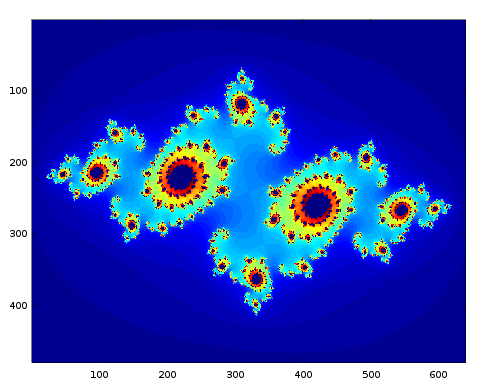
\includegraphics[width = 0.6\textwidth]{img/JuliaOctave.png}
\caption{Conjunto de Julia obtenido mediante octave}
\label{fig:JuliaOctave}
\end{figure}

\subsection{Ejemplos gráficos de explorar el conjunto de Mandelbrot}
El siguiente fragmento de código permite dibujar conjuntos de Mandelbrot con octave

\lstinputlisting{mandelbrot.m}

Ejecutando el fragmento de código tal cual se muestra obtenemos la imagen representada en la figura \ref{fig:MandelbrotOctave}
\begin{figure}[hbtp]
\centering
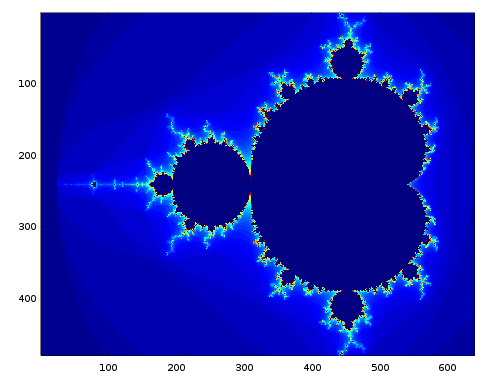
\includegraphics[width = 0.6\textwidth]{img/mandelbrotOctave.png}
\caption{Conjunto de Mandelbrot obtenido mediante octave}
\label{fig:MandelbrotOctave}
\end{figure}

\subsection{Caos y criptografía}
\subsection{Compresión fractal}
La compresión fractal es una tecnología bastante controvertida, con detractores y admiradores. La idea básica detrás de la compresión fractal de imágenes, es expresar la imagen como un sistema de funciones iteradas (IFS). La imagen puede mostrarse rápidamente, y un zoom proporciona infinitos niveles de detalles fractales (sintéticos).

El problema es cómo generar eficientemente la imagen IFS.

Hay cuatro características de la tecnología IFS que es necesario conocer para entender su situación actual:
\begin{itemize}
\item Es un método de compresión que pierde un poco de información (como JPG).
\item La resolución al agrandar es poderosa, pero no una forma de comprimir 100:1.
\item La compresión es lenta, la descompresión es rápida.
\item La tecnología está patentada.
\end{itemize}

Dado que los fractales matemáticos servían para generar imágenes que se veían naturales, se pensó que también podría servir en el sentido opuesto: para comprimirlas.

La idea es tomar una imagen y llevarla a un sistema de funciones iterado, que podría generar el original. No obstante este problema aun no se ha resuelto.

Fue Barnsley, quien en 1988 anunció al mundo que \textbf{si} lo había resuelto, patentando la tecnología. El problema fue que tomaba alrededor de 100 horas para codificar una imagen, y alrededor de 30 minutos para decodificarla, con una persona guiando el proceso. El resultado era una compresión 10.000:1. Poco después con uno de sus alumnos de doctorado, desarrolló un sistema para representar imágenes llamado \textbf{Sistema de Funciones Iteradas Particionado (PIFS)}. Se trataba de un algoritmo que comprimía automáticamente la imagen en un \emph{Sistema de Funciones Iterado Particionado}. El algoritmo no era sofisticado, ni rápido, pero si automático. El costo fue que una imagen codificado con colores de 24-bit podía ser comprimida de 8:1 a 50:1, lo cual aún es bastante bueno.

Todos los programas actuales de compresión de imágenes fractales (que no son muchos) se basan es este algoritmo. La empresa ``Iterated Systems", vende el único compresor/decompresor comercial, llamado ``Images Incorporated". También hay varios programas de académicos disponibles gratuitamente en Internet.

Actualmente la técnica de compresión fractal no supera el estándar de compresión de imágenes JPEG ni el JPEG2000.

\subsection{Antenas fractales}

En la pasada década, los científicos han comenzado a aplicar los fractales a un tema algo \emph{oscuro}: el diseño de las antenas.

Las antenas parecen ser simples, pero la teoría que tienen detrás, basadas en las ecuaciones de Maxwell del electromagnetismo, son impenetrables. Como resultado, los ingenieros de antenas tienen que usar el método de prueba y error. Incluso los mejores y más tecnológicos receptores dependen habitualmente de un hilo que no es mejor que el que usó Marconi para la radio hace cien años.

Los fractales ayudan de dos formas. Primero, pueden mejorar el funcionamiento de los conjuntos de antenas. Muchas antenas parecen estar compuestas de una unidad independiente, incluyendo la mayoría de antenas de radar, pero en realidad están compuestas de formaciones de cientos de pequeñas antenas. Tradicionalmente, estas antenas individuales se colocan de forma aleatoria o de forma ordenada pero Dwight Jaggard, de la Universidad de Pensilvana, junto con otras personas, han descubierto que una colocación en forma de fractal puede combinar la robustez de una colocación aleatoria con la eficiencia de una ordenación coherente, con una reducción significativa del número de elementos necesarios.

``Los fractales son el puente que llena los hueco", comenta Jaggard, ``tienen un desorden a corto alcance y un orden a largo alcance". Incluso las antenas independientes se benefician de tener una forma fractal. Nathan Cohen, un radio astrónomo de la Universidad de Boston, ha experimentado con los cables fractales, conocidos como curvas Koch o triángulos de Sierpinski. No sólo se puede meter la misma longitud de antena en una sexta parte del área, sino que las formas angulares generan capacidades eléctricas y conductividad, eliminando el inconveniente de que los componentes externos sintonicen la antena entre el rango de frecuencias a las que responden.

El por qué las antenas fractales funcionen tan bien fue probado matemáticamente por Cohen y Robert Hohlfeld, quienes establecieron que una buena antena fractal debe satisfacer dos condiciones
\begin{enumerate}
\item Tiene que ser simétrica con respecto a un punto
\item Tiene que ser similar a sí misma (es decir, tener el mismo aspecto básico en cada escala), para poder ser fractal.
\end{enumerate}

Posiblemente, en un futuro cercano, estas antenas fractales tendrán un uso masivo en el nuevo \textbf{Sistema de Identificación por Radiofrecuencia} que sustituirá a los códigos de barras habituales.

\subsection{Aeronáutica y fluidos}

%%%%%%%%%%%%%%%%%%%%%%%%%%%%%
%%%%%%
%%%%%%
%%%%%%
%%%%%%%%%%%%%%%%%%%%%%%%%%%%%
\newpage

\begin{thebibliography}{1}
\bibitem{B1165 SPR}Dprott, J.C, Elegant Chaos
\bibitem{C4260 PEI}Peitgen, H-O, Richter, P.H., The Beauty of Fractals.
\bibitem{B1165 NEW}Hall, Nina, Guide to Chaos
\bibitem{B0240 STR}Strogatz, S.H. Nonlinear Dynamics and Chaos,
\bibitem{B1165 ALL}Alligood, K.T. et al, CHAOS: An introduction to dynamical systems
\end{thebibliography}

\end{document}